% Original thought-experiment sequence; sign convention (-,+,+,+).
\documentclass[11pt,aspectratio=169]{beamer}
\usetheme[progressbar=foot]{moloch}
\usepackage{amsmath,tikz}
\usetikzlibrary{arrows.meta,decorations.pathmorphing}
\definecolor{SpacetimeInk}{HTML}{172B4D}
\setbeamercolor{frametitle}{fg=white,bg=SpacetimeInk}
\setbeamercolor{progress bar}{fg=orange!80!yellow}
\setbeamertemplate{navigation symbols}{}
\title{Gravity as clock comparison}
\subtitle{From a local experiment to a spacetime metric}
\author{Relativity discussion seminar}
\date{Thought experiments 06}
\begin{document}
\maketitle
\section{Compare}
\begin{frame}{Two identical clocks, two different heights}
\framesubtitle{Predict the comparison before writing the metric}
\begin{columns}[c]
\begin{column}{.45\textwidth}
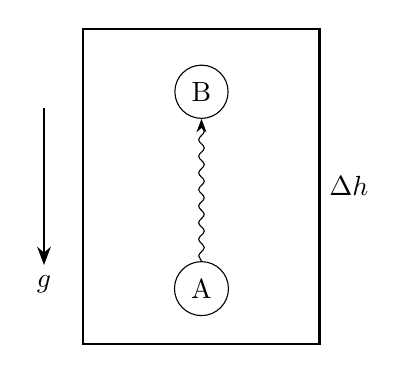
\begin{tikzpicture}[>=Stealth]
\draw[thick] (0,0) rectangle (3,4);
\node[draw,circle] (a) at (1.5,.7) {A};
\node[draw,circle] (b) at (1.5,3.2) {B};
\draw[->,decorate,decoration={snake,amplitude=1pt,segment length=6pt}] (a)--(b);
\node[right] at (3,2) {$\Delta h$};
\draw[->,thick] (-.5,3)--(-.5,1) node[below]{$g$};
\end{tikzpicture}
\end{column}
\begin{column}{.5\textwidth}
\begin{block}{Question}
A clock at A sends regularly spaced light pulses upward. How does B compare the received pulse rate with its own clock?
\end{block}
Specify how the two clocks are held stationary.
\end{column}
\end{columns}
\note{Keep clock rates separate from the frequency of an individual photon. Ask what apparatus maintains the stationary configuration.}
\end{frame}
\begin{frame}{The equivalence principle is local}
\begin{itemize}[<+->]
\item A sufficiently small freely falling laboratory removes a uniform gravitational field from local experiments.
\item Relative acceleration between nearby freely falling objects can remain.
\item That tidal comparison is evidence about curvature.
\end{itemize}
\begin{alertblock}{Do not overextend the elevator}
A local inertial coordinate system is not a global removal of gravity.
\end{alertblock}
\end{frame}
\section{Describe}
\begin{frame}{Write the convention before using the interval}
\framesubtitle{Metric signature $(-,+,+,+)$; $x^0=ct$}
\[
 ds^2=g_{\mu\nu}\,dx^\mu dx^\nu,\qquad d\tau^2=-\frac{ds^2}{c^2}
\]
for timelike worldlines.
\medskip
For a stationary clock in a static weak field,
\[
 g_{00}\simeq-\left(1+\frac{2\Phi}{c^2}\right),
 \qquad d\tau\simeq\left(1+\frac{\Phi}{c^2}\right)dt.
\]
The coordinate time $t$ is shared by this static description; proper time is measured along each clock's worldline.
\end{frame}
\begin{frame}{Compare the rates, not the coordinate labels}
For stationary clocks at potentials $\Phi_A$ and $\Phi_B$,
\begin{align*}
 \frac{d\tau_B}{d\tau_A}
 &\simeq\frac{1+\Phi_B/c^2}{1+\Phi_A/c^2}\\
 &\simeq1+\frac{\Phi_B-\Phi_A}{c^2}.
\end{align*}
\pause
\begin{exampleblock}{Near a uniform terrestrial field}
$\Phi_B-\Phi_A\simeq g\Delta h$. The higher stationary clock accumulates more proper time per common coordinate-time interval.
\end{exampleblock}
\end{frame}
\begin{frame}{A free trajectory extremizes proper time locally}
\[
 \frac{d^2x^\mu}{d\tau^2}
 +\Gamma^\mu_{\alpha\beta}
 \frac{dx^\alpha}{d\tau}\frac{dx^\beta}{d\tau}=0.
\]
\begin{columns}[T]
\begin{column}{.48\textwidth}\begin{block}{Connection}
The Christoffel symbols depend on coordinates; they are not themselves a tensor.
\end{block}\end{column}
\begin{column}{.48\textwidth}\begin{block}{Curvature}
Tidal comparisons need derivatives and combinations of the connection.
\end{block}\end{column}
\end{columns}
\end{frame}
\section{Challenge}
\begin{frame}{Three statements: defend one, repair two}
\begin{enumerate}
\item Gravity can always be removed everywhere by changing coordinates.
\item A coordinate acceleration by itself measures curvature.
\item Proper-time comparisons require specified worldlines.
\end{enumerate}
\bigskip
\uncover<2->{The third statement is the defensible one. Repair the first two by stating what is local and what is coordinate dependent.}
\end{frame}
\begin{frame}[plain]{One picture to carry away}
\centering\Large
A metric tells clocks and rulers\par
how to compare infinitesimal intervals.
\bigskip
\normalsize Geometry earns its meaning through an operational comparison.
\end{frame}
\appendix
\begin{frame}{Reading and conventions}
\small
\begin{thebibliography}{9}
\bibitem{tong} David Tong. \emph{General Relativity}, Chapter 1: Geodesics in Spacetime.
\href{https://www.damtp.cam.ac.uk/user/tong/gr/grhtml/S1.html}{Cambridge lecture notes}.
\end{thebibliography}
This original sequence uses a static weak-field approximation and neglects terms of order $(\Phi/c^2)^2$. The clock sketch is conceptual and carries no experimental data.
\end{frame}
\end{document}
